\documentclass{bioinfo}
\copyrightyear{2020} \pubyear{2020}
% \usepackage{graphicx}
% \usepackage{hyperref}
\access{Advance Access Publication Date: Day Month Year}
\appnotes{Application Note}

\begin{document}
\firstpage{1}

% \subtitle{Subject Section}

\title[short Title]{pyconsFold: Ab initio modelling and docking using distance contact predictions}
\author[Sample \textit{et~al}.]{Lamb, J\,$^{\text{\sfb 1,2}}$, Elofsson, A\,$^{\text{\sfb 1,2}*}$}
\address{$^{\text{\sf 1}}$ Science for Life Laboratory, Stockholm University, SE-171 21 Solna, Sweden\\
$^{\text{\sf 2}}$Department of Biochemistry and Biophysics, Stockholm University, SE-106 91 Stockholm, Sweden}

\corresp{$^\ast$To whom correspondence should be addressed.}

\history{Received on XXXXX; revised on XXXXX; accepted on XXXXX}

\editor{Associate Editor: XXXXXXX}

\abstract{\textbf{Summary:} Contact predictions within a protein are most commonly used in tertiary model prediction of protein structure. Using predicted distance distributions has been shown in many cases to be superior to only using a binary contact annotation, either in contact or not.
pyconsFold builds on the CNS NMR modelling program \cite{Brunger1998-ji,Brunger2007-ut} to use contact predictions as restraints for use in modelling. It builds on the popular CONFOLD-perl \cite{Adhikari2015-fl} script and is rewritten in python both with ease of install, reproducibility and longevity in mind. The package also includes utilities for handling distance predictions from trRosetta \cite{Yang1496} and Quality Assessment tools together with a new novel way of using predicted interprotein contacts to dock two separate protein chains. In contrast to most other folding protocols in use today that uses different approaches of deep learning, pyconsFold builds around the CNS NMR system that is mainly used to fold proteins from NMR spectroscopy data and where the full folding of predicted contacts is the same as the folding when using experimental data.\\
\textbf{Availability and implementation:} pyconsFold is implemented in Python 3 with a strong focus on using as few dependencies as possible for longevity. It is available both as a pip package in Python 3 and as source code on \href{https://github.com/johnlamb/pyconsfold}{github} and is published under the Gnu GPL v3 license.\\
\textbf{Contact:} \href{arne@bioinfo.se}{arne@bioinfo.se}\\
\textbf{Supplementary information:} The full source code together with further documentation and examples are available from \href{https://github}{https://github.com/johnlamb/pyconsfold}.}

\maketitle

\section{pyconsFold}
Protein modelling has long relied on contact predictions that have been presented in binary format, two residues are either in contact (within 8Å) or not. More and more methods are now leveraging full contact distance predictions and this shows (CASP13 \cite{Kryshtafovych2019-zb,Yang1496}) a higher accuracy of the models than if binary contacts were used. 
CONFOLD is a wrapper around CNS that uses predicted binary contacts together with predicted secondary structure to model proteins. pyconsFold is a reimplementation and extension of CONFOLD that achieves better results using distance predictions and that also expands to allow for more geometric restraints, such as angles predicted by tools such as trRosetta and for fast iteration of models and parameters.

pyconsFold has three major modes:

\subsection{Contact based modelling}
Contact based modelling works by treating contacts as an upper limit to distances. CONFOLD style modelling can be replicated using this mode with contact prediction and secondary structure prediction as input and setting the gaps parameter to 5(only use contacts that are at least 5 residues away from each other).

\subsection{Distance based modelling}
Distance based modelling works similar to classical modelling but in this case, an extra column is expected in the CASP-contacts file which defines the standard error for the predicted distance of the contact. By default this mode includes contacts within 5 residues from each other and does not require a secondary structure file. Benchmark has even shown that this mode does not produce better models with a secondary structure file.

\subsection{Docking modelling}
Docking modelling uses CNSs underlying ability to model two protein chains simultaneously. A contact prediction file of both inter and intra contacts needs to be supplied. This can be achieved by running alignment tools for the two chains separately, concatenating these files horizontally and then treating this resulting alignment as one chain and using any contact prediction method to predict contacts. This contact file together with the original fasta files are used as inputs and models the full binary complex.

%\enlargethispage{12pt}
\begin{figure}%[!tpb]%figure1
  \centerline{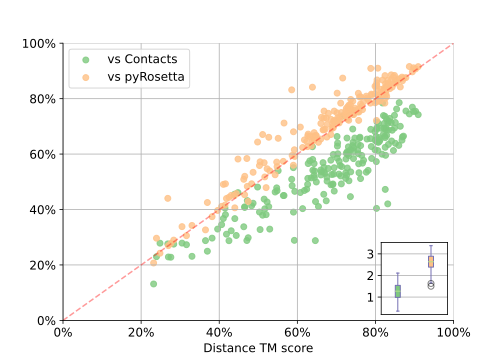
\includegraphics[width=\linewidth]{pyconsFold_figure}}
\caption{pyconsFold distance prediction against both contact base (green) and pyRosetta (orange) models. Distance predictions outperforms contact based predictions in almost all cases. pyconsFolds distance predicted models perform almost as well as pyRosetta but is around 20 times (more than 1 order of magnitude) faster per model as the inset shows(log10 scale of per model time in seconds. pyconsFold in green and pyRosetta in orange).}\label{fig:01}
\end{figure}

\section{Additional features}
For ease of use and reproducibility we have included several extra features and utilities. By default the generated models are ranked by CNS internal NOE energy but Quality Assessment score from pcons \cite{Lundstrom2008-wa} will also be calculated. If a native structure is known and supplied with the tmscore\_pdb\_file argument, the tmscore \cite{Zhang2007-xu,Xu2010-vu} for each model against the native structure will be calculated. 
Compiled versions of both pcons and TMscore for unix based x64 systems are packaged together with pyconsFold under the open source Boost license. If your system does not support the built in versions, you can manually install them on your system and as long as they are in your path, wil be chosen instead of the built in binaries.
l

\section{Conclusion}
pyconsFold offers a complete toolkit for ab initio modelling using predicted contact distances and angles. Its focus is on ease of use and reproducibility and is available both as source on github and as an easily installable pip package in Python 3. It comes packaged with QA-programs to rank the generated models and allows transparency for many tweakable parameters for the underlying CNS-system. It also offers a docking protocol where predicted inter chain contacts are used as restraints for docking. It offers a significant increase in accuracy over contact based protocols by using predicted distances. It is also around 20 times faster than pyRosetta per model.

%%%%%%%%%%%%%%%%%%%%%%%%%%%%%%%%%%%%%%%%%%%%%%%%%%%%%%%%%%%%%%%%%%%%%%%%%%%%%%%%%%%%%
%
%     please remove the " % " symbol from \centerline{\includegraphics{fig01.eps}}
%     as it may ignore the figures.
%
%%%%%%%%%%%%%%%%%%%%%%%%%%%%%%%%%%%%%%%%%%%%%%%%%%%%%%%%%%%%%%%%%%%%%%%%%%%%%%%%%%%%%%

\section*{Acknowledgements}
This work was supported by grants from 
the Swedish Research Council (VR-NT 2016-03798 to A.E.),
National Science Centre (No. 2012/07/E/NZ1/01900 to J.I.S. and
No. 2018/29/N/NZ2/02897 to A.I.J.).
  \subsection*{Conflict of Interest Statement}
  None delared.

% \bibliographystyle{unsrt}
\bibliographystyle{natbib}
%\bibliographystyle{achemnat}
%\bibliographystyle{plainnat}
%\bibliographystyle{abbrv}
%\bibliographystyle{bioinformatics}
%
%\bibliographystyle{plain}
%
\bibliography{references.bib}

\end{document}
